\subsection{Sezione Tecnico}
\label{sec:sezTecnico}

\subsubsection*{Avviso}
Per accedere alle funzionalità del Tecnico è necessario effettuare il login con successo. Le credenziali di accesso sono:
\begin{itemize}
    \item \textbf{Nome utente} (username): admin;
    \item \textbf{Password}: admin. 
\end{itemize}

\subsubsection{Autenticazione} \label{sec:autenticazione}
Nella sezione superiore destra dell'interfaccia, cliccando sull'icona di login 
\includegraphics[height=1.2em]{assets/user_icon.png}, l'Utente può inserire le credenziali per sbloccare le funzionalità del Tecnico.
\begin{figure}[H]
  \centering
  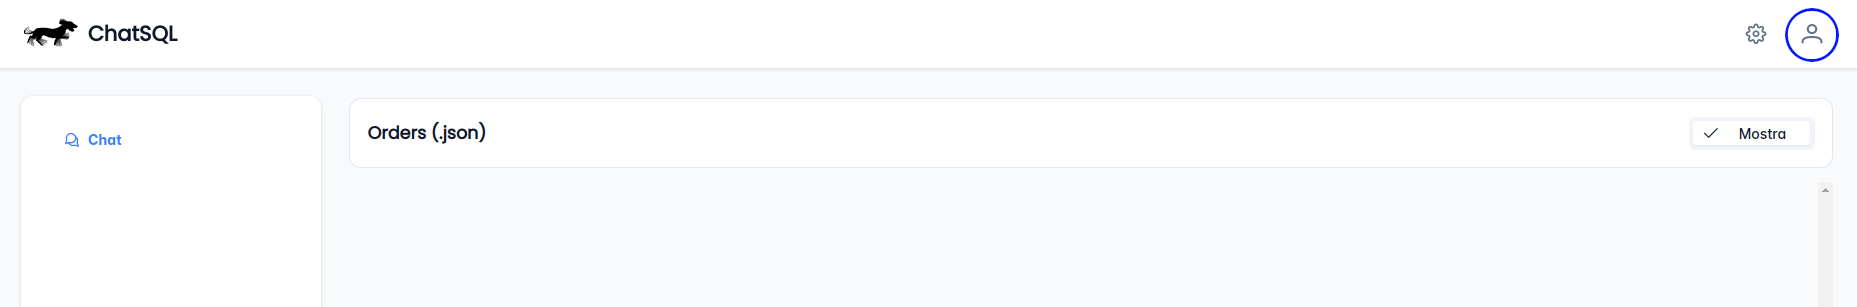
\includegraphics[width=1\textwidth]{assets/login_topbar.png}
  \caption{Topbar con menu di autenticazione}
\end{figure}
\begin{figure}[H]
  \centering
  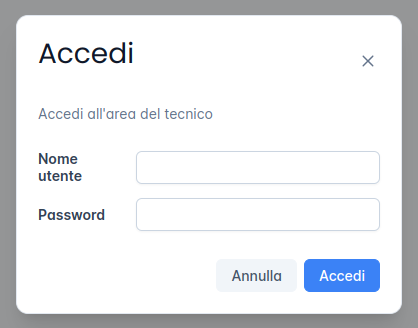
\includegraphics[width=0.50\textwidth]{assets/login_modal.png}
  \caption{Modale di login}
\end{figure}

\subsubsection{Gestione dizionari}
\begin{figure}[H]
  \centering
  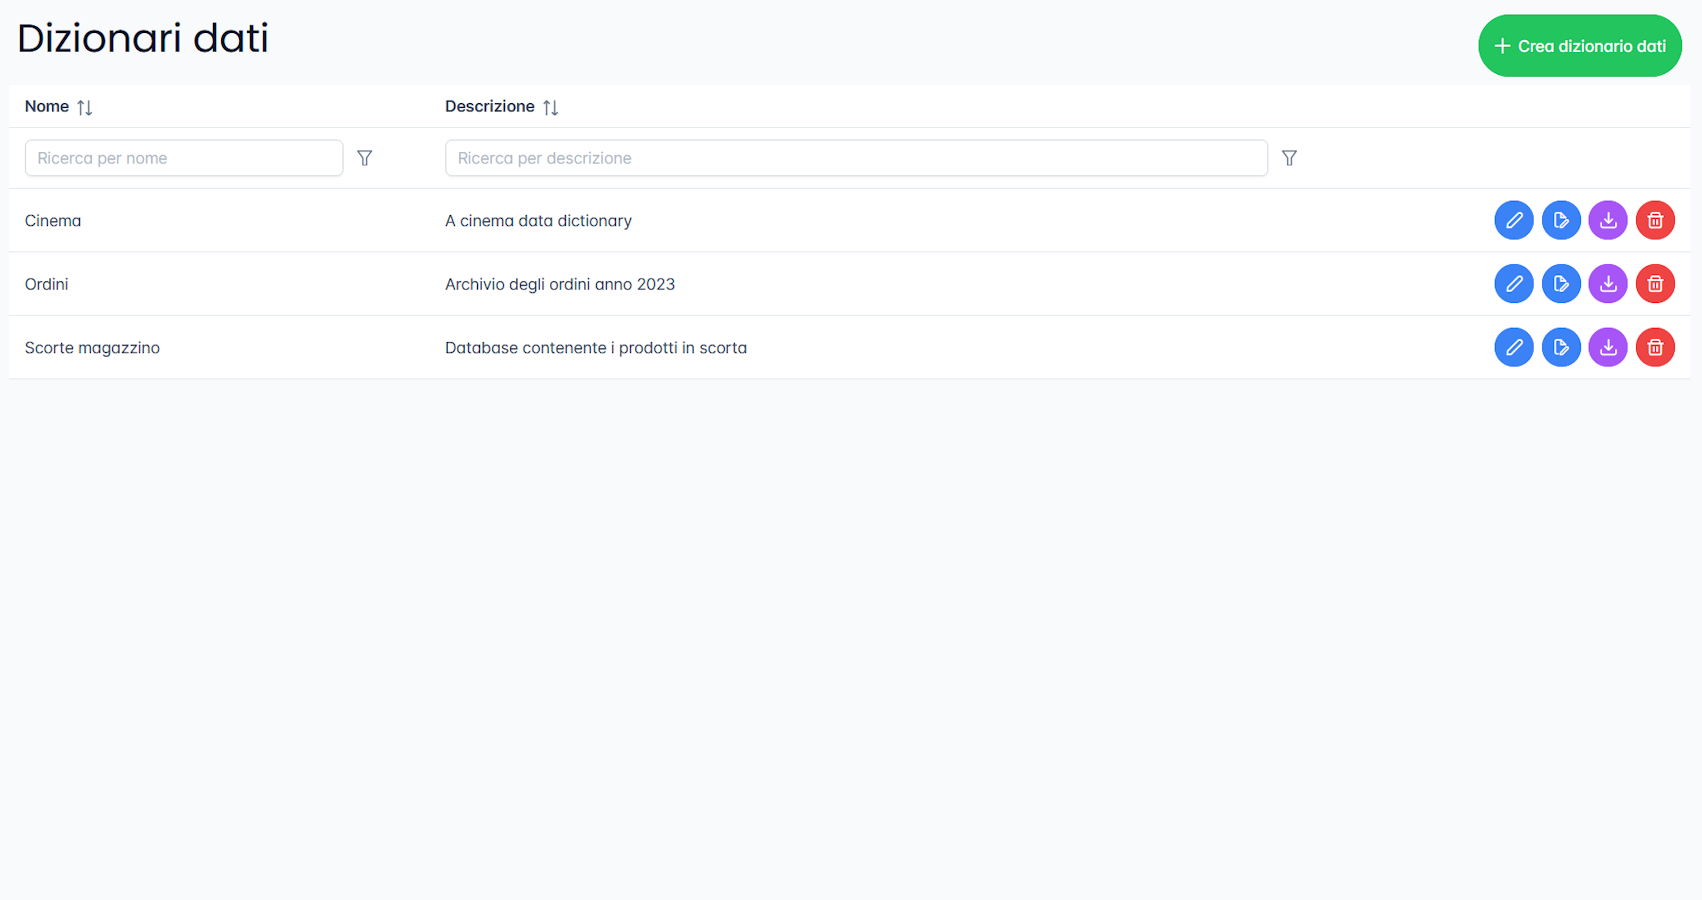
\includegraphics[width=1\textwidth]{assets/dd_list.png}
  \caption{Schermata di gestione dizionari dati}
\end{figure}
\par La schermata soprastante mostra la lista completa dei \glossario{dizionari dati} caricati nel sistema. Vengono fornite le funzionalità per operare su di essi.

\subsubsubsection{Inserimento dizionario dati}
Cliccando sul pulsante "Crea dizionario dati" 
\includegraphics[height=1.2em]{assets/dd_create_button.png} si aprirà una modale dove sarà possibile inserire i parametri di un nuovo \glossario{dizionario dati}:
\begin{figure}[H]
  \centering
  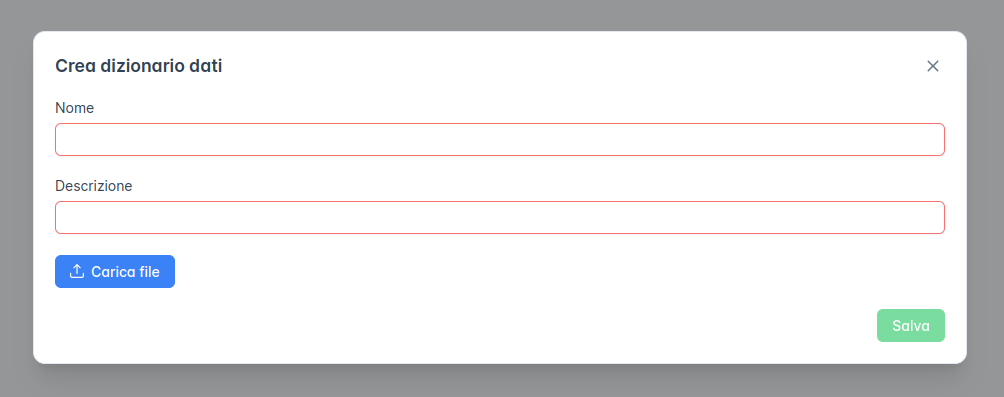
\includegraphics[width=0.5\textwidth]{assets/dd_modal_create.png}
  \caption{Modale di creazione dizionario dati}
\end{figure}
\begin{itemize}
  \item \textbf{Nome}: deve essere univoco rispetto agli altri dizionari dati;
  \item \textbf{Descrizione}: stringa testuale che descrive brevemente il dizionario dati;
  \item \textbf{File}: deve essere un file in formato JSON, di dimensione massima 1 MB e strutturato secondo il modello proposto.
\end{itemize}
\vspace{0.5\baselineskip}
\par Al salvataggio il dizionario verrà aggiunto alla lista.

\subsubsubsection{Aggiornamento dizionario dati}
Cliccando sul pulsante di aggiornamento dei metadati 
\includegraphics[height=1.2em]{assets/dd_edit_metadata_button.png} si aprirà una modale dove sarà possibile modificare i parametri:
\begin{itemize}
  \item \textbf{Nome}: deve essere univoco rispetto agli altri \glossario{dizionari dati};
  \item \textbf{Descrizione}: stringa testuale che descrive brevemente il dizionario dati.
\end{itemize}

\subsubsubsection{Modifica file di configurazione dizionario dati}
Cliccando sul pulsante di modifica del file di configurazione di un \glossario{dizionario dati} 
\includegraphics[height=1.2em]{assets/dd_edit_button.png} si aprirà una modale dove sarà possibile caricare un nuovo file.

\subsubsubsection{Scarica file dizionario dati}
Cliccando sul pulsante di download 
\includegraphics[height=1.2em]{assets/dd_download_button.png} verrà scaricato il file del \glossario{dizionario dati} corrispondente in formato JSON.

\subsubsubsection{Elimina file dizionario dati}
Cliccando sul pulsante di cancellazione 
\includegraphics[height=1.2em]{assets/dd_delete_button.png} si aprirà una modale di conferma per l'eliminazione del \glossario{dizionario dati}.
\begin{figure}[H]
  \centering
  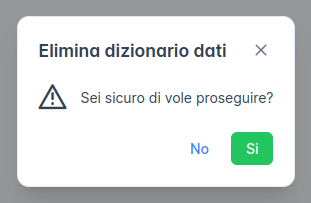
\includegraphics[width=0.5\textwidth]{assets/dd_confirm_delete.png}
  \caption{Modale di conferma eliminazione dizionario dati}
\end{figure}
In caso di conferma il dizionario verrà eliminato dalla lista.

\subsubsection{Strumento di debug}

\subsubsubsection{Generazione del messaggio di debug}
\par Per il Tecnico è disponibile uno strumento di controllo per i meccanismi di generazione del \glossario{prompt} che aiuta a comprendere e analizzare i passaggi algoritmici che hanno prodotto il prompt restituito sulla base di una interrogazione. Il \glossario{debug} assiste il Tecnico nella fase di miglioramento del \glossario{dizionario dati}, poiché fornisce una panoramica dell'interazione tra i modelli di intelligenza artificiale e il dizionario stesso. L'obiettivo di questa funzionalità è individuare le aree del dizionario dati che necessitano di aggiornamenti, con particolare attenzione alle descrizioni in linguaggio naturale di tabelle e colonne.

\par Per utilizzare questa funzionalità, il Tecnico deve inserire un messaggio nell'apposita maschera di richiesta all'interno della chat (sezione utente 6.1). Una volta ottenuto il prompt, è necessario cliccare l'icona del punto interrogativo in alto a destra, da cui si aprirà un'altra finestra sovrapposta a quella attuale.

\begin{figure}[H]
  \centering
  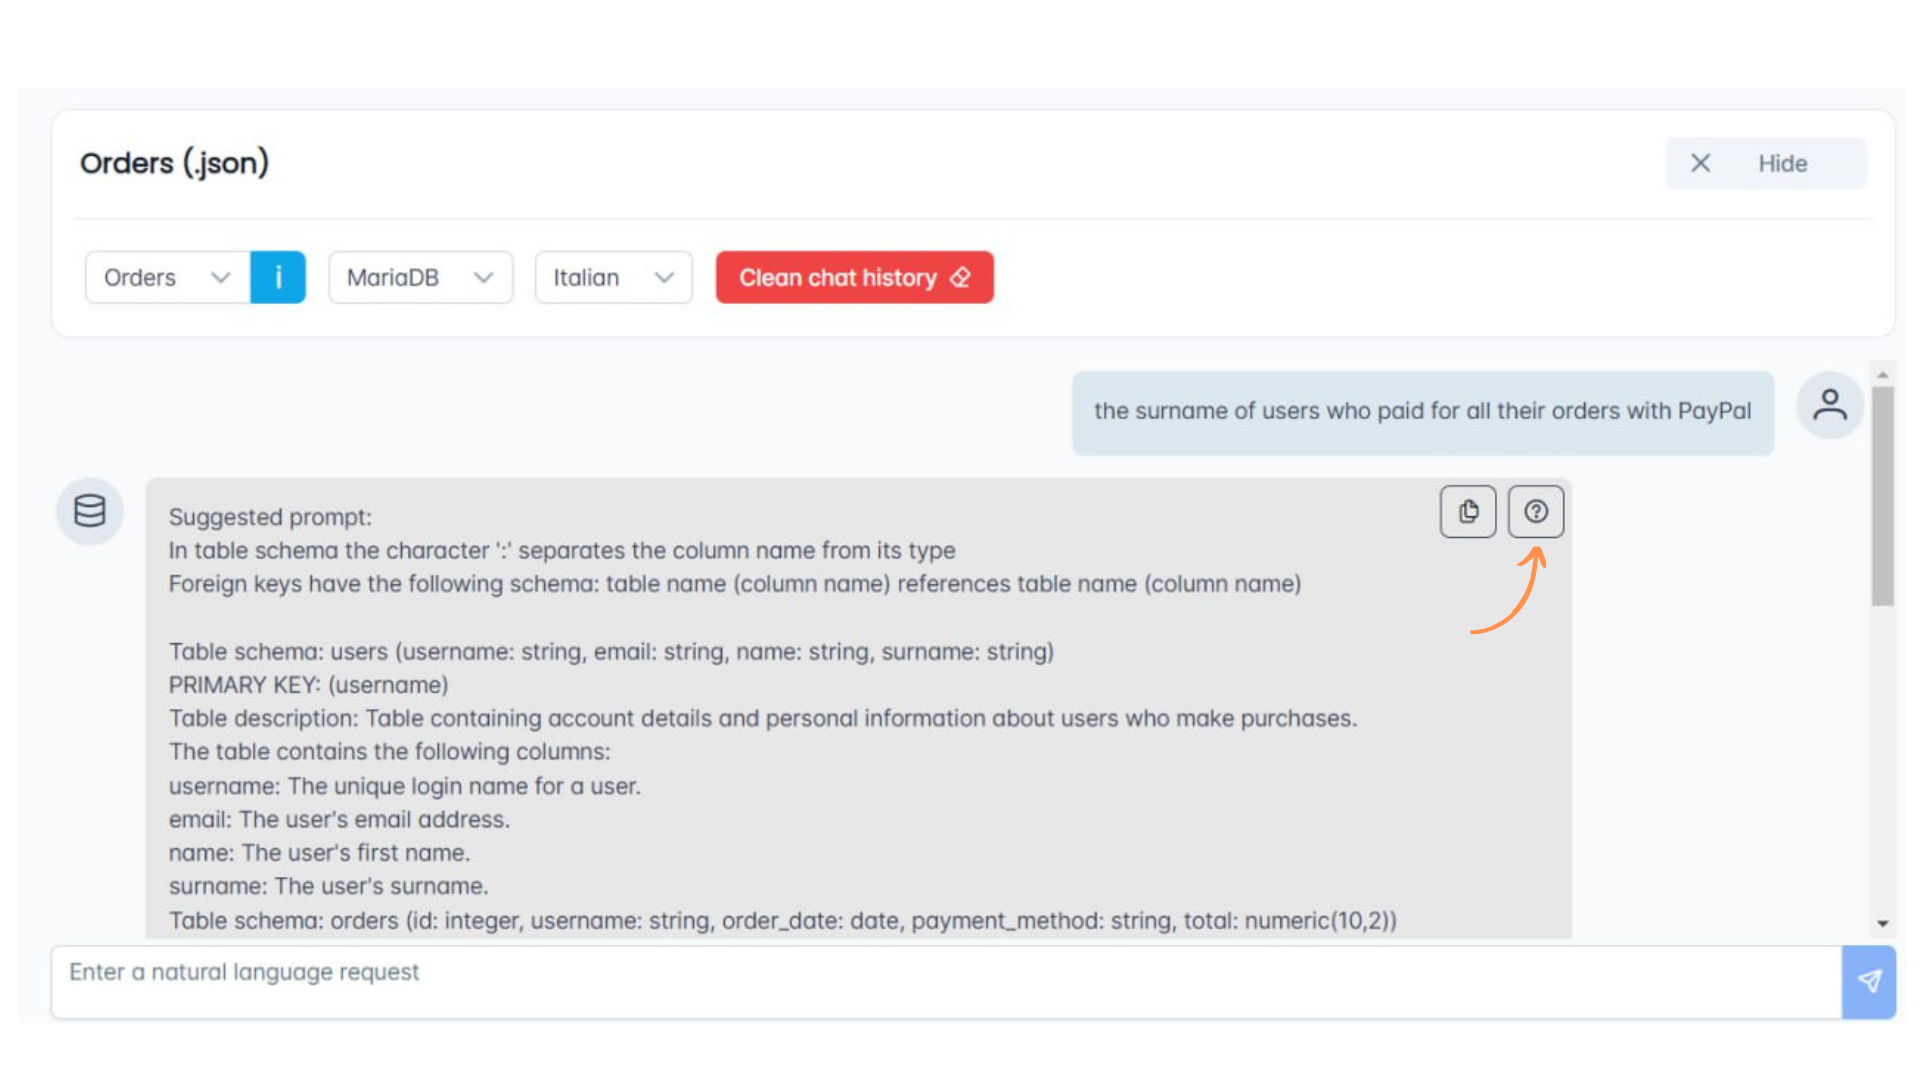
\includegraphics[width=\textwidth]{assets/tasto_info_debug.png}
  \caption{Selezione funzionalità di debug}
\end{figure}

\par Nel messaggio di debug è documentato il modo in cui le descrizioni interagiscono con il modello di \glossario{AI}. In ordine verranno visualizzate le seguenti informazioni: 
\begin{itemize}
  \item Data e ora di generazione del \glossario{log}; 
  \item La richiesta inserita in linguaggio naturale;
  \item Analisi della prima fase della generazione del prompt con una lista delle tabelle considerate rilevanti dal modello, di cui si riportano le seguenti informazioni:
  \begin{itemize}
    \item Nome della tabella;
    \item Punteggio assegnato alla tabella;
    \item Descrizione della tabella;
    \item Classifica di importanza dei termini presenti nella descrizione della tabella;
    \item Descrizione della colonna più rilevante;
    \item Classifica di importanza dei termini presenti nella descrizione della colonna.
  \end{itemize}
  \item Analisi della seconda fase di generazione del prompt con una lista delle tabelle pertinenti, di cui viene indicato il motivo per cui sono state inserite o meno nel prompt finale.
\end{itemize}
\begin{figure}[H]
  \centering
  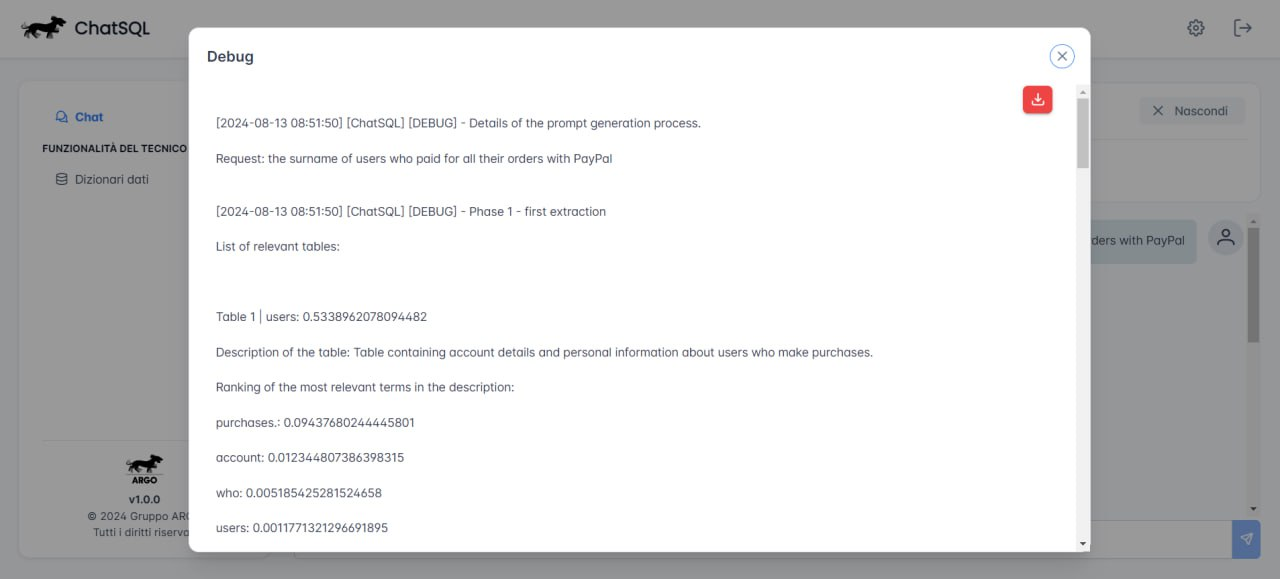
\includegraphics[width=\textwidth]{assets/analisi_debug1.jpg}
\end{figure}

\begin{figure}[H]
  \centering
  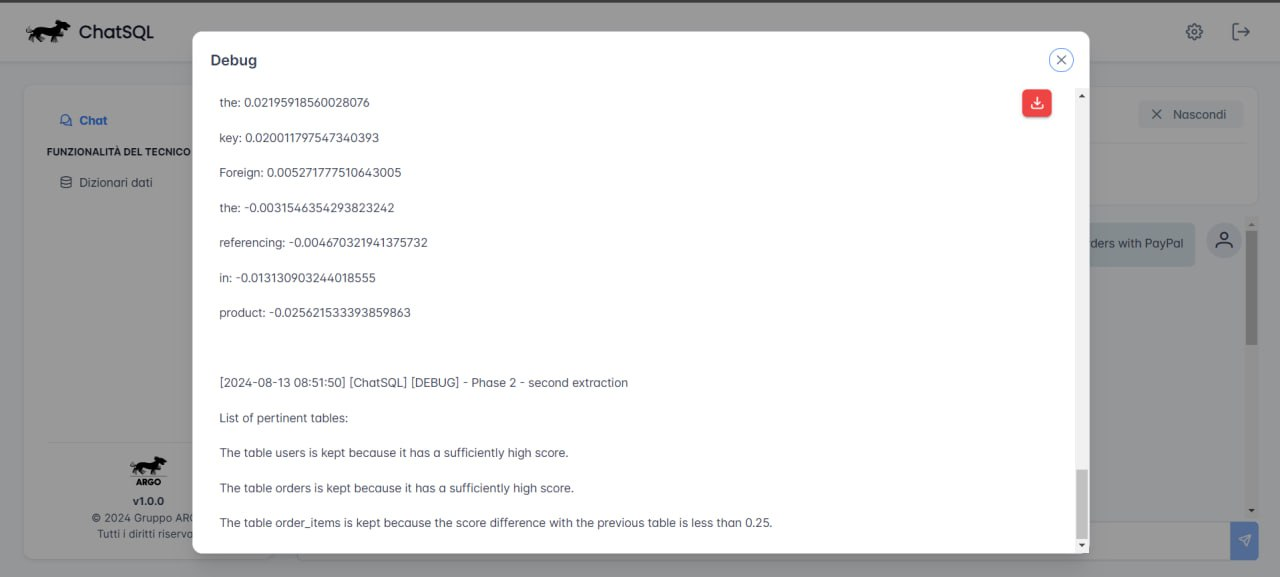
\includegraphics[width=\textwidth]{assets/analisi_debug2.jpg}
  \caption{Esempio di messaggio prodotto}
\end{figure}

\par Cliccando il pulsante di chiusura in alto a destra, il modale di debug verrà nascosto e sarà possibile visualizzare nuovamente il prompt generato.
\begin{figure}[H]
  \centering
  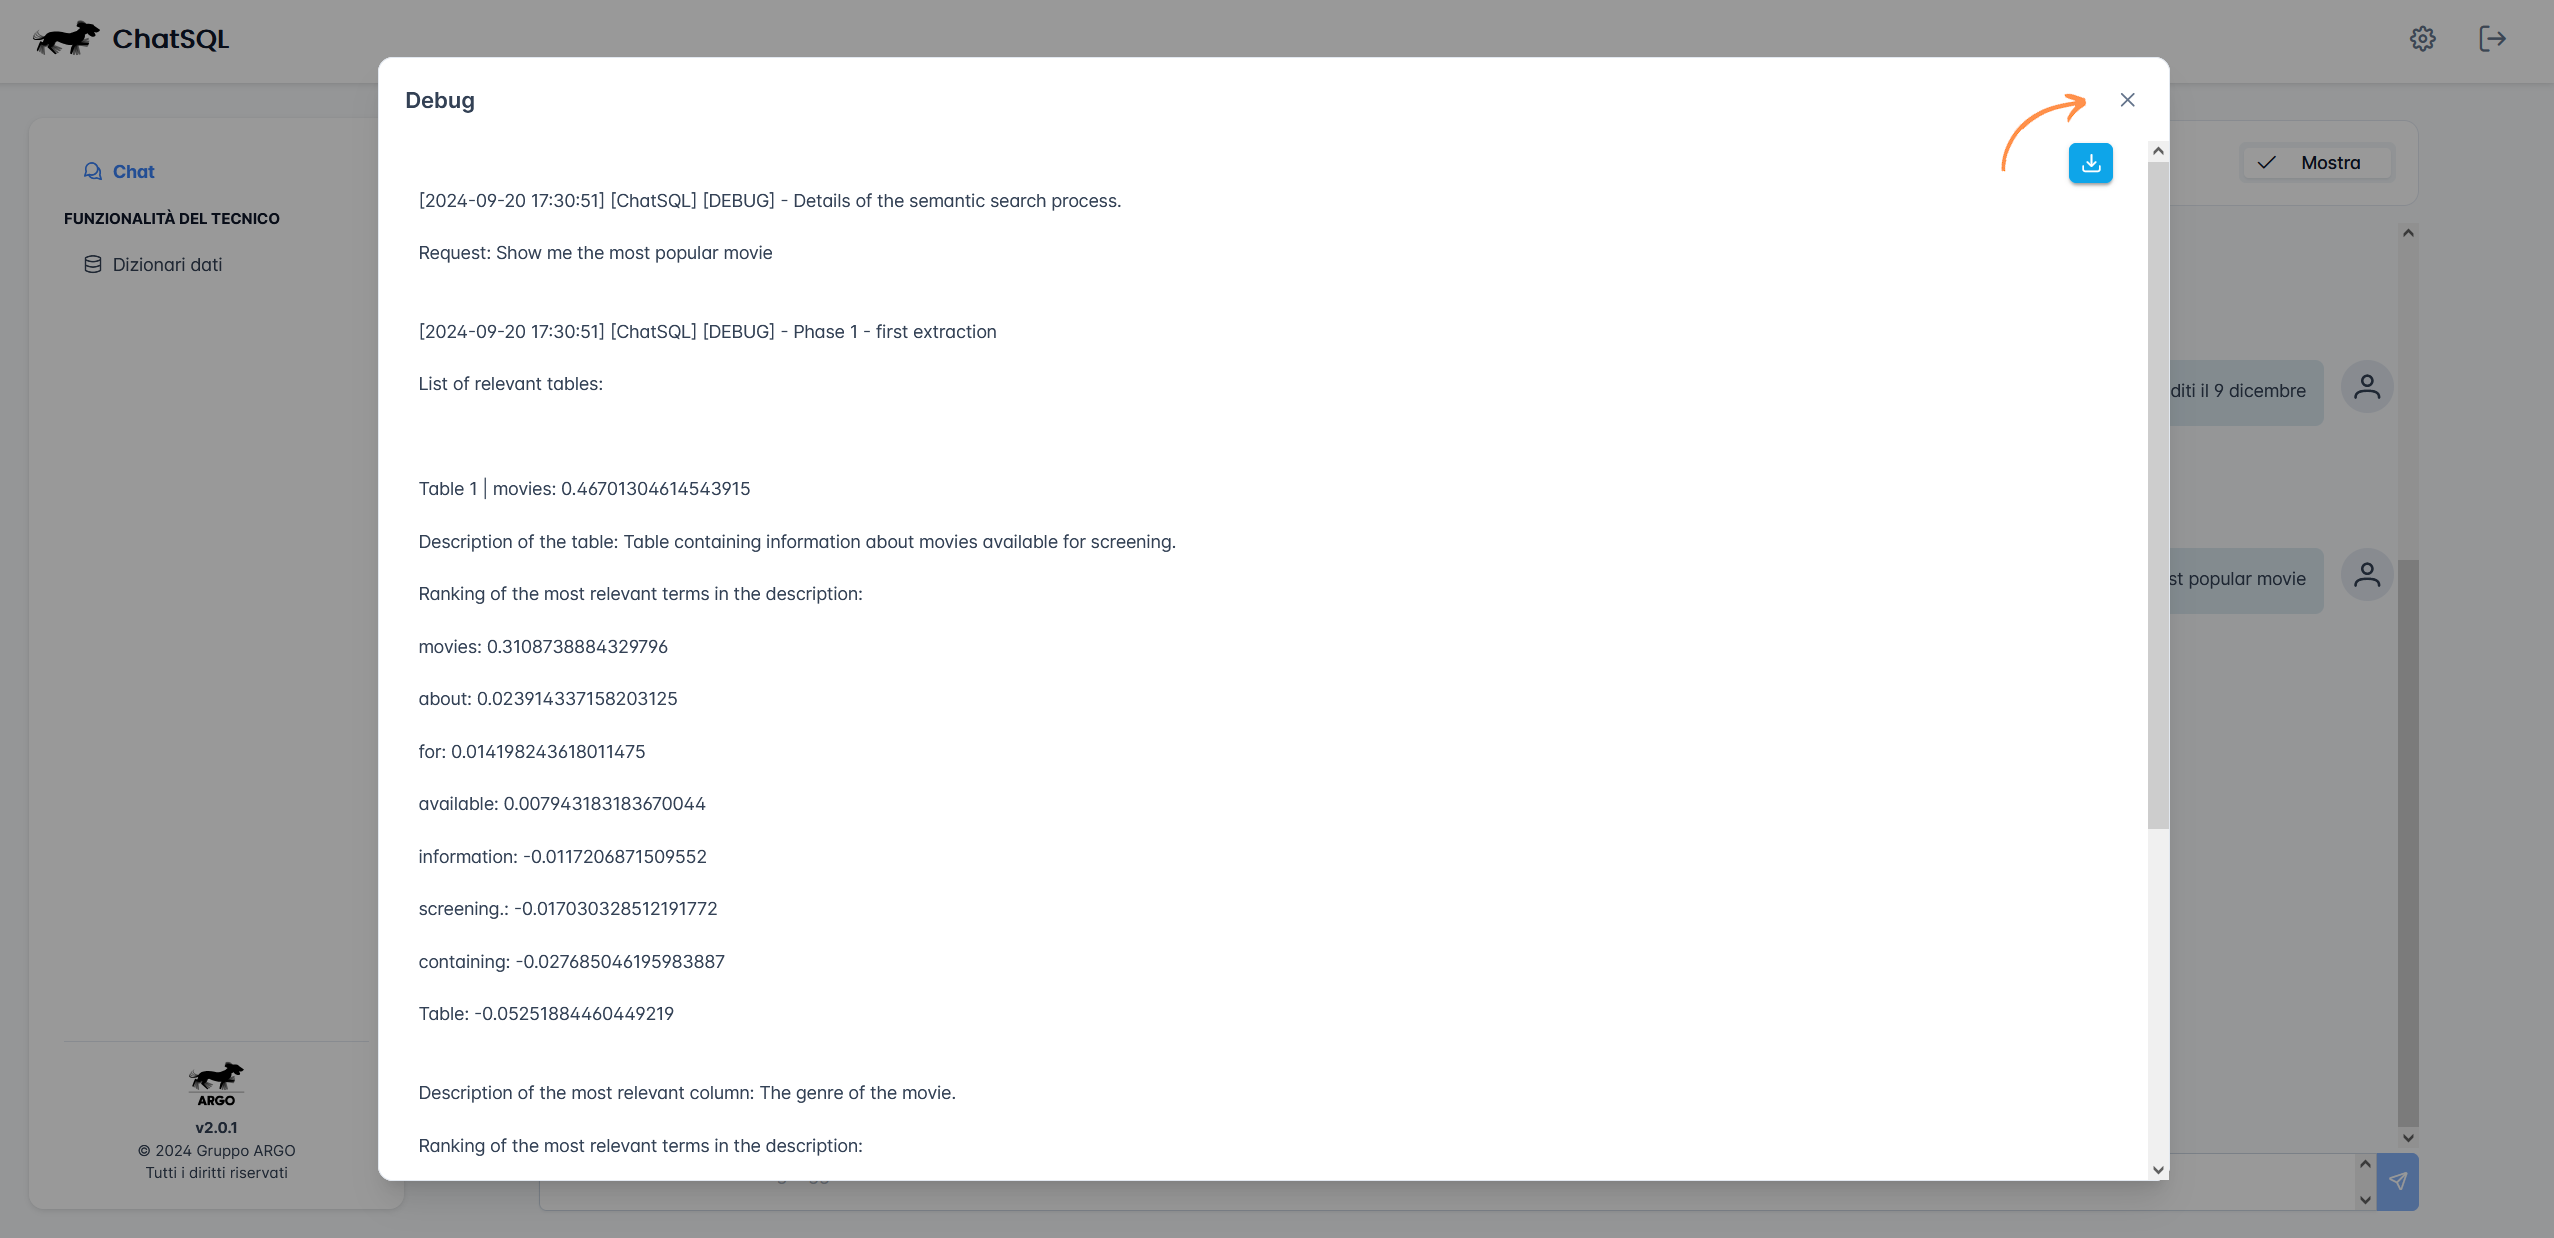
\includegraphics[width=\textwidth]{assets/tasto_close_debug.png}
  \caption{Icona chiusura messaggio di debug}
\end{figure}

\subsubsubsection{Download del messaggio di debug}

Il messaggio di debug può essere scaricato in formato \textit{txt}, in modo da conservarlo in locale e utilizzarlo per migliorare il \glossario{dizionario dati} o per produrre analisi a posteriori.
\begin{figure}[H]
  \centering
  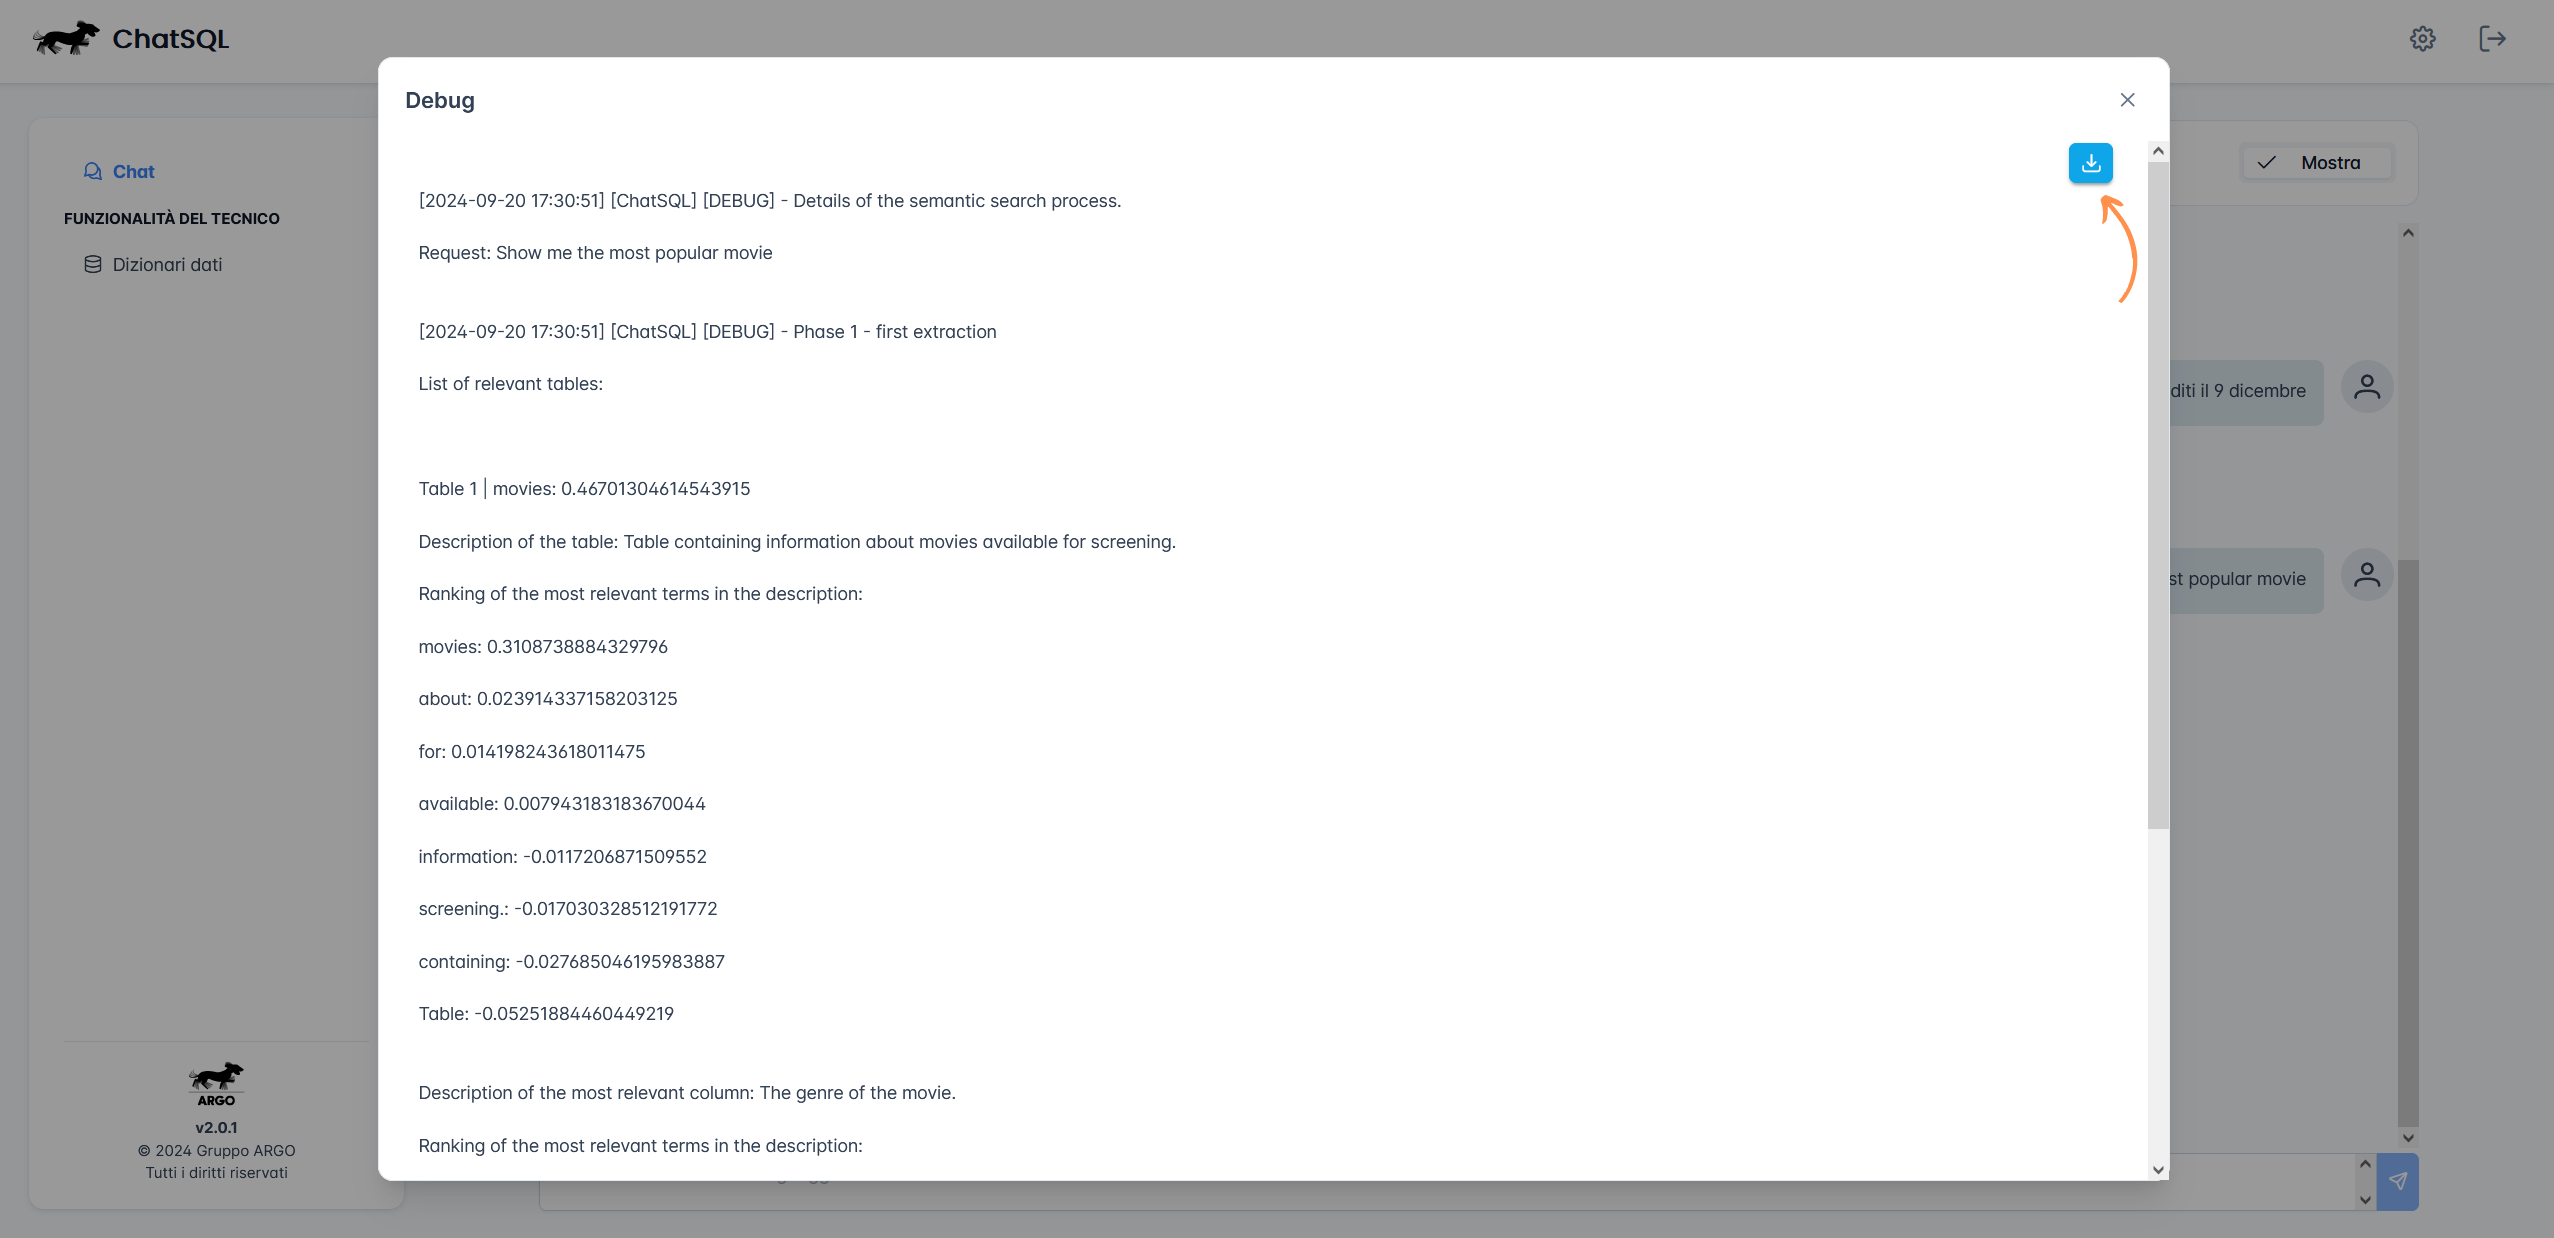
\includegraphics[width=\textwidth]{assets/tasto_dawnload_debug.png}
  \caption{Download del messaggio di debug}
\end{figure}





